\chapter{Database Design and Relational Modeling}

\section{Introduction}
A marketplace platform handling real-time room bookings, peer-to-peer product orders, in-app chat messages, and student behavioral telemetry requires a dependable relational database. The data persistence layer must guarantee ACID (Atomicity, Consistency, Isolation, Durability) transactions so that rooms and products are never oversold, foreign key constraints are strictly preserved, and queries execute swiftly under concurrent browsing.

StayMart uses \textbf{MySQL 8.0} with the transactional \textbf{InnoDB} storage engine. InnoDB provides row-level locking, foreign key constraint enforcement, and native JSON column support, allowing structured listing attributes (such as amenity lists and photo URLs) to be stored alongside normalized relational data without requiring complex table joins for simple read queries.

This chapter details StayMart's database design:
\begin{enumerate}
    \item Entity-Relationship (ER) modeling and domain relationships.
    \item Data dictionaries for all twelve normalized relational tables.
    \item Normalization analysis demonstrating compliance with 1NF, 2NF, 3NF, and BCNF.
    \item Indexing strategy and referential integrity constraints.
\end{enumerate}

\section{Entity-Relationship (ER) Modeling}
Figure \ref{fig:erd_model} illustrates the complete Entity-Relationship diagram for the StayMart database schema.

\begin{figure}[htbp]
    \centering
    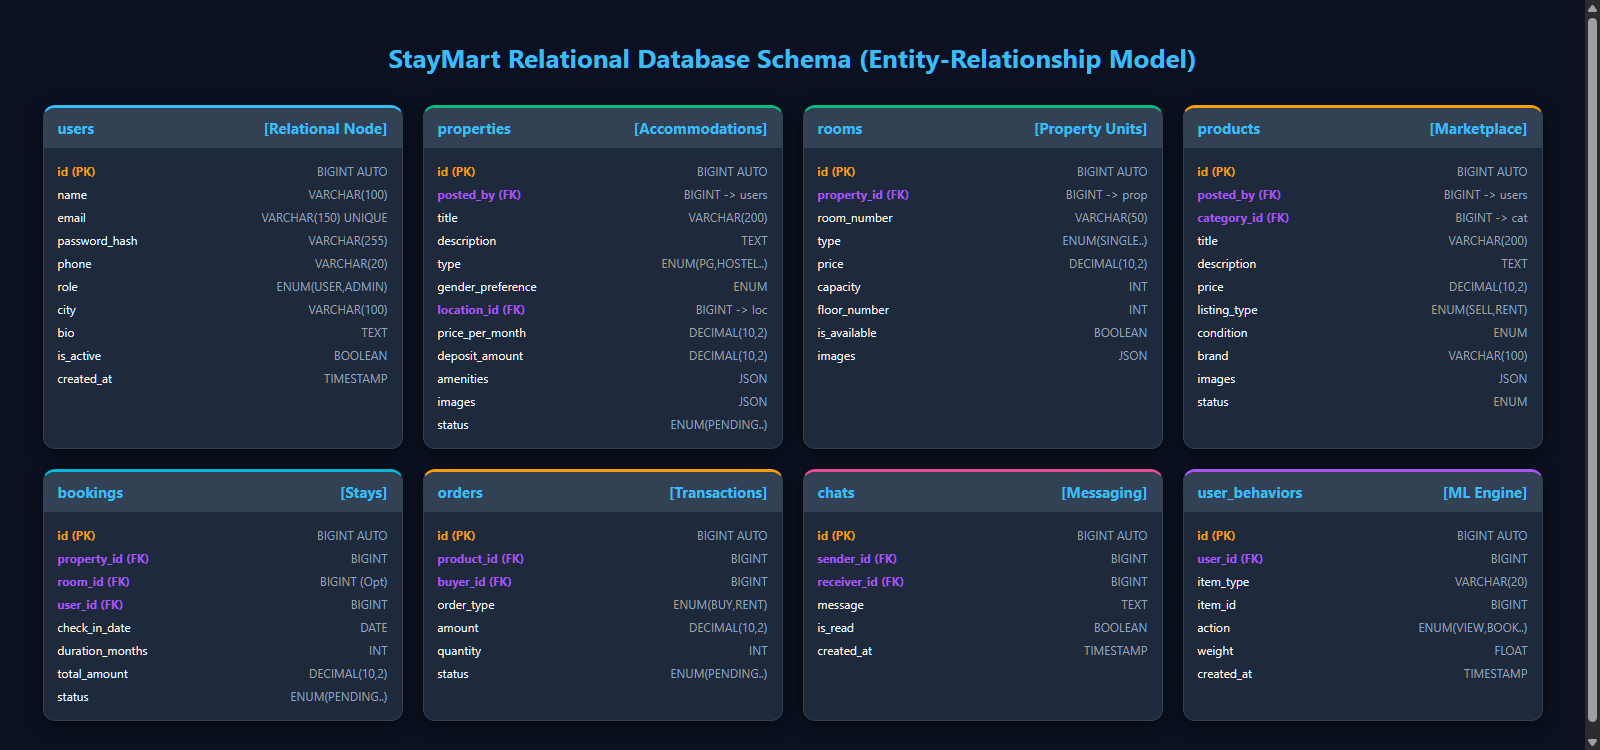
\includegraphics[width=0.98\textwidth]{diagrams/er_diagram.png}
    \caption{Entity-Relationship (ER) Diagram of the StayMart Relational Database Schema}
    \label{fig:erd_model}
\end{figure}

The schema models key relationships across the student marketplace:
\begin{itemize}
    \item \textbf{Users to Properties ($1:N$):} A registered user can list multiple accommodations (\texttt{properties.posted\_by}).
    \item \textbf{Properties to Rooms ($1:N$):} An accommodation contains one or more discrete room configurations (\texttt{rooms.property\_id}) representing single, double, triple, or dormitory beds with individual rent rates.
    \item \textbf{Locations to Listings ($1:N$):} Standardized geographic location records (\texttt{locations.id}) link to properties and products, enforcing consistent city, area, and coordinate data.
    \item \textbf{Categories to Products ($1:N$):} Products belong to hierarchical categories (\texttt{categories.id}) such as Electronics, Mobile Phones, Furniture, Books, and Appliances.
    \item \textbf{Users to Bookings and Orders ($1:N$):} A student submits accommodation bookings (\texttt{bookings.booker\_id}) and classified purchase/rental orders (\texttt{orders.buyer\_id}).
    \item \textbf{Users to Peer Chat ($N:M$ via \texttt{chats}):} Bilateral communication is recorded in \texttt{chats}, linking \texttt{sender\_id} and \texttt{receiver\_id} with listing context.
    \item \textbf{Users to Behavioral Events ($1:N$):} Telemetry events (views, searches, wishlists, booking attempts) are captured in \texttt{user\_behaviors} to train the recommendation engine.
\end{itemize}

\section{Relational Schema Data Dictionaries}
The StayMart schema comprises twelve tables with explicit data types, default values, and foreign key constraints.

\subsection{Table: \texttt{users}}
Stores registered user accounts, contact information, role assignments, and profile details.
\begin{table}[htbp]
\centering
\caption{Data Dictionary: \texttt{users} Table}
\label{tab:dict_users}
\footnotesize
\begin{tabularx}{\textwidth}{lp{2.8cm}lp{2.2cm}X}
\toprule
\textbf{Column Name} & \textbf{Data Type} & \textbf{Nullability} & \textbf{Default} & \textbf{Description} \\
\midrule
\texttt{id} & \texttt{BIGINT} & NOT NULL & AUTO\_INCR & Primary Key, unique user identifier. \\
\texttt{name} & \texttt{VARCHAR(100)} & NOT NULL & None & Full name of the student or property host. \\
\texttt{email} & \texttt{VARCHAR(150)} & NOT NULL & None & Unique login email address. \\
\texttt{password\_hash} & \texttt{VARCHAR(255)} & NOT NULL & None & BCrypt password hash ($cost=10$). \\
\texttt{phone} & \texttt{VARCHAR(15)} & NULL & NULL & Contact phone number for inquiries. \\
\texttt{role} & \texttt{ENUM} & NOT NULL & 'USER' & Role: \texttt{USER} or \texttt{ADMIN}. \\
\texttt{city} & \texttt{VARCHAR(100)} & NULL & 'Dehradun' & Primary campus city in Uttarakhand. \\
\texttt{state} & \texttt{VARCHAR(100)} & NULL & 'Uttarakhand' & State jurisdiction. \\
\texttt{bio} & \texttt{TEXT} & NULL & NULL & User bio or caretaker description. \\
\texttt{profile\_pic} & \texttt{VARCHAR(255)} & NULL & NULL & Relative or remote URL to avatar image. \\
\texttt{is\_active} & \texttt{BOOLEAN} & NOT NULL & TRUE & Account active/suspended flag. \\
\texttt{is\_verified} & \texttt{BOOLEAN} & NOT NULL & FALSE & Verification badge indicator. \\
\texttt{created\_at} & \texttt{TIMESTAMP} & NOT NULL & CURRENT\_TS & Account creation timestamp. \\
\bottomrule
\end{tabularx}
\end{table}

\subsection{Table: \texttt{locations}}
Geographic taxonomy representing cities and student campus clusters across Uttarakhand.
\begin{table}[htbp]
\centering
\caption{Data Dictionary: \texttt{locations} Table}
\label{tab:dict_locations}
\footnotesize
\begin{tabularx}{\textwidth}{lp{2.8cm}lp{2.2cm}X}
\toprule
\textbf{Column Name} & \textbf{Data Type} & \textbf{Nullability} & \textbf{Default} & \textbf{Description} \\
\midrule
\texttt{id} & \texttt{BIGINT} & NOT NULL & AUTO\_INCR & Primary Key, location identifier. \\
\texttt{city} & \texttt{VARCHAR(100)} & NOT NULL & None & City name (e.g., Dehradun, Rishikesh, Roorkee). \\
\texttt{area} & \texttt{VARCHAR(100)} & NULL & NULL & Specific campus locality (e.g., Clement Town). \\
\texttt{state} & \texttt{VARCHAR(100)} & NULL & 'Uttarakhand' & State name. \\
\texttt{pincode} & \texttt{VARCHAR(10)} & NULL & NULL & Postal code. \\
\texttt{latitude} & \texttt{DECIMAL(10,8)} & NULL & NULL & Latitude coordinate. \\
\texttt{longitude} & \texttt{DECIMAL(11,8)} & NULL & NULL & Longitude coordinate. \\
\bottomrule
\end{tabularx}
\end{table}

\subsection{Table: \texttt{categories}}
Product and accommodation taxonomy organizing listings into intuitive browsing buckets.
\begin{table}[htbp]
\centering
\caption{Data Dictionary: \texttt{categories} Table}
\label{tab:dict_categories}
\footnotesize
\begin{tabularx}{\textwidth}{lp{2.8cm}lp{2.2cm}X}
\toprule
\textbf{Column Name} & \textbf{Data Type} & \textbf{Nullability} & \textbf{Default} & \textbf{Description} \\
\midrule
\texttt{id} & \texttt{BIGINT} & NOT NULL & AUTO\_INCR & Primary Key, category identifier. \\
\texttt{name} & \texttt{VARCHAR(100)} & NOT NULL & None & Category name (e.g., Electronics, Furniture). \\
\texttt{type} & \texttt{ENUM} & NOT NULL & None & Category type: \texttt{ACCOMMODATION} or \texttt{PRODUCT}. \\
\texttt{icon} & \texttt{VARCHAR(50)} & NULL & NULL & Icon identifier or CSS class name. \\
\texttt{parent\_id} & \texttt{BIGINT} & NULL & NULL & Foreign Key $\rightarrow$ \texttt{categories(id)} (self-reference). \\
\bottomrule
\end{tabularx}
\end{table}

\subsection{Table: \texttt{properties}}
Rental accommodation listings including PGs, hostels, shared flats, and rooms.
\begin{table}[htbp]
\centering
\caption{Data Dictionary: \texttt{properties} Table}
\label{tab:dict_properties}
\footnotesize
\begin{tabularx}{\textwidth}{lp{2.8cm}lp{2.2cm}X}
\toprule
\textbf{Column Name} & \textbf{Data Type} & \textbf{Nullability} & \textbf{Default} & \textbf{Description} \\
\midrule
\texttt{id} & \texttt{BIGINT} & NOT NULL & AUTO\_INCR & Primary Key, property listing ID. \\
\texttt{posted\_by} & \texttt{BIGINT} & NOT NULL & None & Foreign Key $\rightarrow$ \texttt{users(id)}. \\
\texttt{title} & \texttt{VARCHAR(200)} & NOT NULL & None & Listing headline. \\
\texttt{description} & \texttt{TEXT} & NULL & NULL & Detailed property description and rules. \\
\texttt{type} & \texttt{ENUM} & NOT NULL & None & PG, ROOM, HOSTEL, HOTEL, FLAT, DORMITORY. \\
\texttt{gender\_preference}& \texttt{ENUM} & NOT NULL & 'ANY' & MALE, FEMALE, or ANY. \\
\texttt{address} & \texttt{VARCHAR(255)} & NULL & NULL & Street address or landmark. \\
\texttt{area} & \texttt{VARCHAR(100)} & NULL & NULL & Local campus area name. \\
\texttt{location\_id} & \texttt{BIGINT} & NULL & NULL & Foreign Key $\rightarrow$ \texttt{locations(id)}. \\
\texttt{price\_per\_month}& \texttt{DECIMAL(10,2)}& NULL & NULL & Base monthly rental rate (INR). \\
\texttt{deposit\_amount} & \texttt{DECIMAL(10,2)}& NOT NULL & 0.00 & Refundable security deposit. \\
\texttt{amenities} & \texttt{JSON} & NULL & NULL & JSON array of amenities (WiFi, Power Backup, Meals). \\
\texttt{total\_rooms} & \texttt{INT} & NOT NULL & 1 & Total capacity / rooms in listing. \\
\texttt{available\_rooms}& \texttt{INT} & NOT NULL & 1 & Currently vacant rooms/beds. \\
\texttt{images} & \texttt{JSON} & NULL & NULL & JSON array of photograph URLs. \\
\texttt{status} & \texttt{ENUM} & NOT NULL & 'PENDING' & PENDING, APPROVED, or REJECTED. \\
\texttt{is\_available} & \texttt{BOOLEAN} & NOT NULL & TRUE & Active availability toggle. \\
\texttt{created\_at} & \texttt{TIMESTAMP} & NOT NULL & CURRENT\_TS & Publication timestamp. \\
\bottomrule
\end{tabularx}
\end{table}

\subsection{Table: \texttt{rooms}}
Individual room configurations within an accommodation property.
\begin{table}[htbp]
\centering
\caption{Data Dictionary: \texttt{rooms} Table}
\label{tab:dict_rooms}
\footnotesize
\begin{tabularx}{\textwidth}{lp{2.8cm}lp{2.2cm}X}
\toprule
\textbf{Column Name} & \textbf{Data Type} & \textbf{Nullability} & \textbf{Default} & \textbf{Description} \\
\midrule
\texttt{id} & \texttt{BIGINT} & NOT NULL & AUTO\_INCR & Primary Key, room identifier. \\
\texttt{property\_id} & \texttt{BIGINT} & NOT NULL & None & Foreign Key $\rightarrow$ \texttt{properties(id)}. \\
\texttt{room\_number} & \texttt{VARCHAR(20)} & NULL & NULL & Room number or identifier label. \\
\texttt{type} & \texttt{ENUM} & NOT NULL & None & SINGLE, DOUBLE, TRIPLE, or DORMITORY. \\
\texttt{price} & \texttt{DECIMAL(10,2)}& NULL & NULL & Monthly rent for this room configuration. \\
\texttt{capacity} & \texttt{INT} & NOT NULL & 1 & Maximum number of student occupants. \\
\texttt{floor\_number} & \texttt{INT} & NOT NULL & 0 & Floor number within building. \\
\texttt{is\_available} & \texttt{BOOLEAN} & NOT NULL & TRUE & Availability status of room. \\
\texttt{images} & \texttt{JSON} & NULL & NULL & JSON array of room-specific photos. \\
\bottomrule
\end{tabularx}
\end{table}

\subsection{Table: \texttt{products}}
Marketplace listings for second-hand student gear posted for sale or rent.
\begin{table}[htbp]
\centering
\caption{Data Dictionary: \texttt{products} Table}
\label{tab:dict_products}
\footnotesize
\begin{tabularx}{\textwidth}{lp{2.8cm}lp{2.2cm}X}
\toprule
\textbf{Column Name} & \textbf{Data Type} & \textbf{Nullability} & \textbf{Default} & \textbf{Description} \\
\midrule
\texttt{id} & \texttt{BIGINT} & NOT NULL & AUTO\_INCR & Primary Key, product listing ID. \\
\texttt{posted\_by} & \texttt{BIGINT} & NOT NULL & None & Foreign Key $\rightarrow$ \texttt{users(id)}. \\
\texttt{category\_id} & \texttt{BIGINT} & NULL & NULL & Foreign Key $\rightarrow$ \texttt{categories(id)}. \\
\texttt{title} & \texttt{VARCHAR(200)} & NOT NULL & None & Item headline (e.g., Symphony Cooler). \\
\texttt{description} & \texttt{TEXT} & NULL & NULL & Item condition, specifications, and reason for selling. \\
\texttt{price} & \texttt{DECIMAL(10,2)}& NOT NULL & None & Asking price or rental rate (INR). \\
\texttt{listing\_type} & \texttt{ENUM} & NOT NULL & 'SELL' & SELL, RENT, or BOTH. \\
\texttt{condition} & \texttt{ENUM} & NOT NULL & 'GOOD' & NEW, LIKE\_NEW, GOOD, FAIR, or OLD. \\
\texttt{brand} & \texttt{VARCHAR(100)} & NULL & NULL & Manufacturer or brand name. \\
\texttt{location\_id} & \texttt{BIGINT} & NULL & NULL & Foreign Key $\rightarrow$ \texttt{locations(id)}. \\
\texttt{area} & \texttt{VARCHAR(100)} & NULL & NULL & Campus area or pickup neighborhood. \\
\texttt{images} & \texttt{JSON} & NULL & NULL & JSON array of authentic item photos. \\
\texttt{status} & \texttt{ENUM} & NOT NULL & 'PENDING' & PENDING, APPROVED, or REJECTED. \\
\texttt{is\_available} & \texttt{BOOLEAN} & NOT NULL & TRUE & Inventory flag (active vs. sold). \\
\texttt{views\_count} & \texttt{INT} & NOT NULL & 0 & Popularity view counter. \\
\texttt{created\_at} & \texttt{TIMESTAMP} & NOT NULL & CURRENT\_TS & Publication timestamp. \\
\bottomrule
\end{tabularx}
\end{table}

\subsection{Tables: \texttt{bookings}, \texttt{orders}, \texttt{wishlists}, \texttt{reviews}, \texttt{chats}, and \texttt{user\_behaviors}}
The remaining transactional and interaction tables are structured as follows:

\begin{itemize}
    \item \textbf{\texttt{bookings}:} Captures accommodation reservations. Foreign keys: \texttt{booker\_id} $\rightarrow$ \texttt{users(id)}, \texttt{property\_id} $\rightarrow$ \texttt{properties(id)}, and optional \texttt{room\_id} $\rightarrow$ \texttt{rooms(id)}. Columns include \texttt{check\_in} (DATE), \texttt{check\_out} (DATE), \texttt{months} (INT), \texttt{total\_amount} (DECIMAL), \texttt{status} (\texttt{PENDING}, \texttt{CONFIRMED}, \texttt{CANCELLED}, \texttt{COMPLETED}), and \texttt{message} (TEXT).
    \item \textbf{\texttt{orders}:} Captures classified product purchases and rentals. Foreign keys: \texttt{buyer\_id} $\rightarrow$ \texttt{users(id)}, \texttt{seller\_id} $\rightarrow$ \texttt{users(id)}, and \texttt{product\_id} $\rightarrow$ \texttt{products(id)}. Columns include \texttt{quantity} (INT), \texttt{amount} (DECIMAL), \texttt{order\_type} (\texttt{BUY} or \texttt{RENT}), \texttt{rent\_start} (DATE), \texttt{rent\_end} (DATE), \texttt{status}, and \texttt{message}.
    \item \textbf{\texttt{wishlists}:} Manages saved student bookmarks. Foreign key: \texttt{user\_id} $\rightarrow$ \texttt{users(id)}. Columns include \texttt{item\_type} (\texttt{PROPERTY} or \texttt{PRODUCT}), \texttt{item\_id} (BIGINT), and a unique constraint on \texttt{(user\_id, item\_type, item\_id)} preventing duplicate bookmarks.
    \item \textbf{\texttt{reviews}:} Stores student ratings and feedback after confirmed stays or purchases. Foreign key: \texttt{reviewer\_id} $\rightarrow$ \texttt{users(id)}. Columns include \texttt{item\_type} (\texttt{PROPERTY}, \texttt{PRODUCT}, or \texttt{USER}), \texttt{item\_id} (BIGINT), \texttt{rating} (INT, constrained between 1 and 5), and \texttt{comment} (TEXT).
    \item \textbf{\texttt{chats}:} Records direct peer-to-peer messages between students and hosts. Foreign keys: \texttt{sender\_id} $\rightarrow$ \texttt{users(id)} and \texttt{receiver\_id} $\rightarrow$ \texttt{users(id)}. Columns include \texttt{listing\_type}, \texttt{listing\_id}, \texttt{message} (TEXT), \texttt{is\_read} (BOOLEAN), and \texttt{timestamp}.
    \item \textbf{\texttt{user\_behaviors}:} Records user telemetry for recommendation model training. Foreign key: \texttt{user\_id} $\rightarrow$ \texttt{users(id)}. Columns include \texttt{item\_type}, \texttt{item\_id}, \texttt{action} (\texttt{VIEW}, \texttt{SEARCH}, \texttt{WISHLIST}, \texttt{BOOK}, \texttt{ORDER}, \texttt{CONTACT}), \texttt{search\_query}, \texttt{city\_filter}, and \texttt{timestamp}.
\end{itemize}

\section{Database Normalization Analysis}
To eliminate data redundancy and prevent insertion, update, and deletion anomalies, we evaluate the schema through formal normalization stages.

\subsection{First Normal Form (1NF)}
A relation satisfies 1NF if all attribute domains contain only atomic, indivisible values, and there are no repeating groups.
\begin{itemize}
    \item Every column in StayMart—such as \texttt{price}, \texttt{name}, \texttt{email}, and \texttt{status}—contains atomic scalar values.
    \item \textbf{Use of JSON Attributes:} Columns like \texttt{amenities} and \texttt{images} in \texttt{properties} and \texttt{products} store JSON arrays. Under MySQL 8.0, the native \texttt{JSON} type functions as an atomic document datatype. Storing image URLs and amenity tags as serialized collections attached to a single listing avoids maintaining separate join tables for static arrays while strictly preserving 1NF.
\end{itemize}

\subsection{Second Normal Form (2NF)}
A relation is in 2NF if it is in 1NF and every non-prime attribute is fully functionally dependent on the entire primary key (no partial key dependencies).
\begin{itemize}
    \item Every table in StayMart uses a single-column surrogate primary key (\texttt{id BIGINT AUTO\_INCREMENT}).
    \item Because every candidate key consists of exactly one attribute ($K = \{\text{id}\}$), a partial dependency on a subset of a composite key is impossible. Therefore, all twelve tables satisfy 2NF unconditionally.
\end{itemize}

\subsection{Third Normal Form (3NF)}
A relation is in 3NF if it is in 2NF and no non-prime attribute is transitively dependent on the primary key. Formally, for every non-trivial functional dependency $X \rightarrow Y$, either $X$ is a superkey or $Y$ is a prime attribute.

\textbf{Practical Case Study: Geographical Normalization (\texttt{locations})} \\
Consider an unnormalized property table containing city, area, and pincode directly:
\begin{equation}
\text{PropertyID} \rightarrow \{\text{Area}, \text{City}, \text{State}, \text{Pincode}\}
\end{equation}
This design introduces transitive dependencies because:
\begin{equation}
\text{PropertyID} \rightarrow \text{Pincode} \quad \text{and} \quad \text{Pincode} \rightarrow \{\text{City}, \text{State}\}
\end{equation}
This causes three classic database anomalies:
\begin{enumerate}
    \item \textbf{Redundancy:} Every student PG in Clement Town would duplicate the string ``Clement Town, Dehradun, Uttarakhand, 248002''.
    \item \textbf{Update Anomaly:} Changing a locality name requires updating hundreds of individual property rows.
    \item \textbf{Deletion Anomaly:} Deleting all listings in a new campus locality would delete the knowledge that the locality exists in the database.
\end{enumerate}

StayMart eliminates this transitive dependency by isolating geographic data into the \texttt{locations} relation. Properties reference \texttt{location\_id} as a foreign key. Thus, all non-prime attributes in \texttt{properties} depend directly on the primary key, satisfying 3NF.

\subsection{Boyce-Codd Normal Form (BCNF)}
A relation is in BCNF if for every non-trivial functional dependency $X \rightarrow Y$, $X$ is a superkey. In StayMart, all non-trivial functional dependencies originate from primary keys (\texttt{id}) or unique candidate keys (such as \texttt{users.email}), which are verified superkeys. Therefore, the schema satisfies BCNF.

\section{Indexing Strategy and Referential Integrity}
To ensure fast query execution across thousands of student listings, B-Tree indexes are defined on foreign keys and search filter columns:

\begin{enumerate}
    \item \textbf{Foreign Key Indexes:} Indexes on \texttt{properties(posted\_by)}, \texttt{properties(location\_id)}, \texttt{products(category\_id)}, \texttt{bookings(property\_id)}, and \texttt{orders(product\_id)} ensure that relational joins execute efficiently via index range scans rather than full table scans.
    \item \textbf{Search Filter Indexes:} The public catalog search frequently filters by approval status and availability. Composite indexes on \texttt{(status, is\_available, created\_at)} allow MySQL to filter approved listings directly from the index tree.
    \item \textbf{Telemetry Stream Indexes:} The \texttt{user\_behaviors} table receives high write volume. An index on \texttt{(user\_id, created\_at)} allows the recommendation service to retrieve a user's recent interactions in milliseconds.
\end{enumerate}

\section{Summary}
This chapter presented the database design of StayMart, detailing the twelve relational tables, ER modeling, normalization proofs, and indexing strategy. The use of MySQL 8.0 with InnoDB guarantees transactional consistency for room bookings and product orders, while native JSON columns efficiently handle media assets and amenity tags. The following chapter details the backend implementation and machine learning recommendation microservice.
